% 
% Lecture Template for ME3050 -  Dynamics Modeling and Controls - Tennessee Technological University
%
% Tristan Hill, % Spring 2020 - Summer 2020
% Module 6->4 - Spring Systems
% Topic 3 - The Mass Spring Model
%

\documentclass{beamer}                         % for presentation (has nav buttons at bottom)
%\documentclass[handout]{beamer}  % for handout 
\usepackage{beamerthemesplit}
\usepackage{amsmath}
\usepackage{listings}
\usepackage{multicol}
\usepackage{framed}

\beamertemplateballitem

% custom colors
\definecolor{TTUpurple}{rgb}{0.3098, 0.1607, 0.5176} % TTU Purple (primary)
\definecolor{TTUgold}{rgb}{1.0000, 0.8666, 0.0000} % TTU Gold (primary) 
\definecolor{mygray}{rgb}{.6, .6, .6}
\definecolor{mypurple}{rgb}{0.6,0.1961,0.8}
\definecolor{mybrown}{rgb}{0.5451,0.2706,0.0745}
\definecolor{mygreen}{rgb}{0, .39, 0}
\definecolor{mypink}{rgb}{0.9960, 0, 0.9960}

% color commands
\newcommand{\R}{\color{red}}
\newcommand{\B}{\color{blue}}
\newcommand{\BR}{\color{mybrown}}
\newcommand{\K}{\color{black}}
\newcommand{\G}{\color{mygreen}}
\newcommand{\PR}{\color{mypurple}}
\newcommand{\PN}{\color{mypink}}
\newcommand{\OR}{\color{TTU}}
\newcommand{\GD}{\color{TTUgold}}

% Beamer colors
\setbeamercolor{palette primary}{bg=TTUpurple,fg=TTUgold}
\setbeamercolor{palette secondary}{bg=black,fg=TTUgold}
\setbeamercolor{palette tertiary}{bg=black,fg=TTUpurple}
\setbeamercolor{palette quaternary}{bg=TTUgold,fg=black}
\setbeamercolor{structure}{fg=TTUpurple} % itemize, enumerate, etc
\setbeamercolor{section in toc}{fg=TTUpurple} % TOC sections

\newcommand{\Lagr}{\mathcal{L}} % lagrangian

\newcommand{\hspcu}{\underline{\hspace{20mm}}} % large horizontal space w underline
\newcommand{\vspccc}{\vspace{6mm}\\} % large vertical space
\newcommand{\vspcc}{\vspace{4mm}\\}   % medium vertical space
\newcommand{\vspc}{\vspace{2mm}\\}     % small vertical space

\newcommand{\hspcccc}{\hspace{10mm}} % large horizontal space
\newcommand{\hspccc}{\hspace{6mm}} % large horizontal space
\newcommand{\hspcc}{\hspace{4mm}}   % medium horizontal space
\newcommand{\hspc}{\hspace{2mm}}     % small horizontal space

\newcommand{\MNUM}{4\hspace{2mm}} % Module number
\newcommand{\TNUM}{3\hspace{2mm}} % Topic number 

\newcommand{\moduletitle}{Spring Systems}
\newcommand{\topictitle}{The Mass Spring Model} 

\newcommand{\sectiontitleI}{Motivation}
\newcommand{\sectiontitleII}{The Mass-Spring Model}
\newcommand{\sectiontitleIII}{Newton's Approach}
\newcommand{\sectiontitleIV}{Example: Automotive Suspension}

% custom box
\newsavebox{\mybox}

\title{Lecture Module - \moduletitle}
\date{Mechanical Engineering\vspc Tennessee Technological University}
\author{ME3050 - Dynamics Modeling and Controls}

\begin{document}

\lstset{language=MATLAB,basicstyle=\ttfamily\small,showstringspaces=false}

\frame{\titlepage \center\begin{framed}\Large \textbf{Topic \TNUM - \topictitle}\end{framed} \vspace{5mm}}

% Section 0: Outline
\frame{

\large \textbf{Topic \TNUM - \topictitle} \vspace{3mm}\\
\begin{multicols}{2}
\begin{itemize}

	\item \sectiontitleI    \vspc % Section I
	\item \sectiontitleII 	\vspc % Section II
	\item \sectiontitleIII 	\vspc %Section III
	\item \sectiontitleIV 	\vspc %Section IV

\end{itemize}
\hspace{10mm}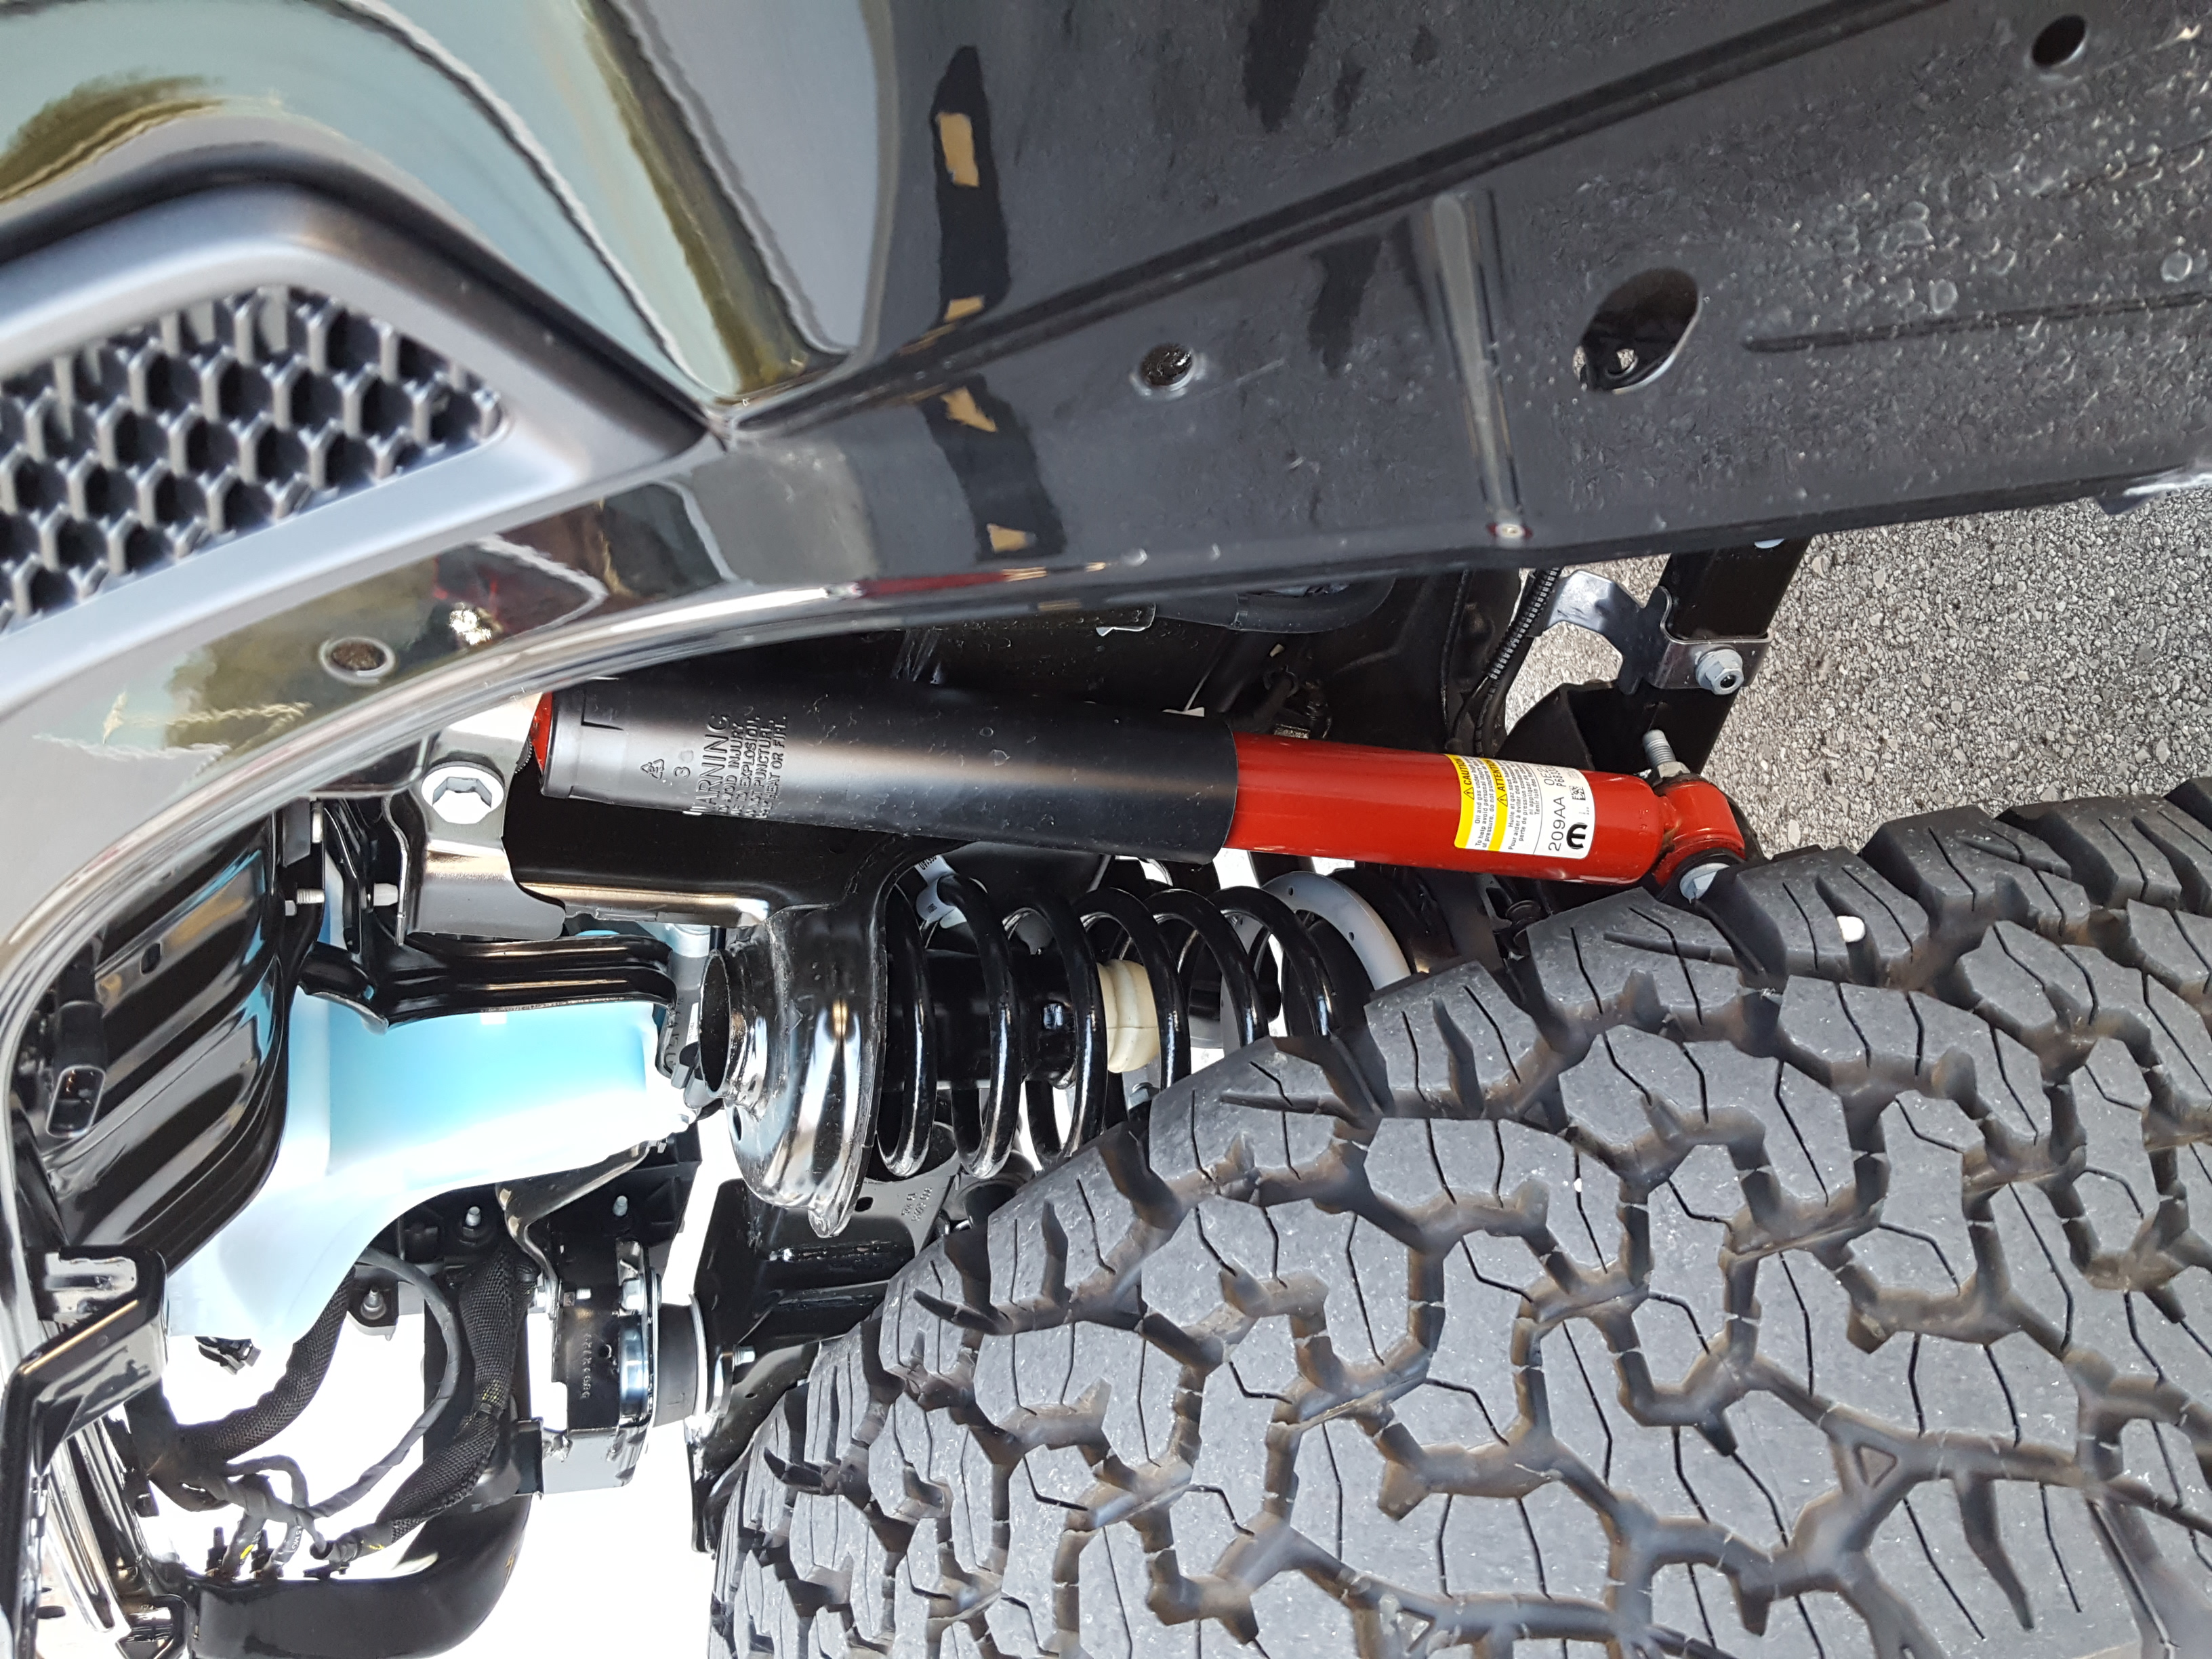
\includegraphics[scale=.04,angle=-90,origin=c]{jeep_02.jpg}
\end{multicols}


}

% Section I
\section{\sectiontitleI}

	% Section I - Frame I
	\frame{
		\frametitle{\sectiontitleI}
		
		\begin{multicols}{2}
		
		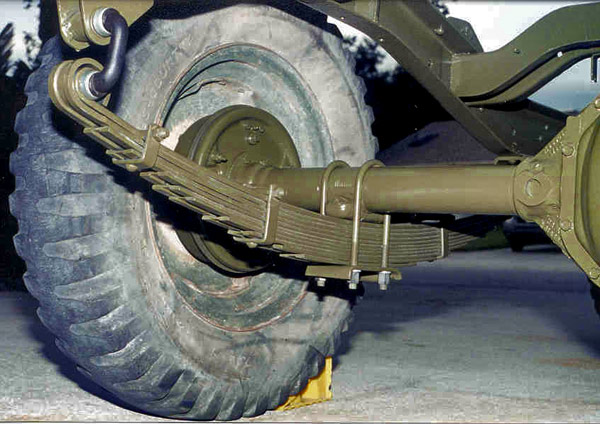
\includegraphics[scale=.25]{leaf_springs.jpg}			
		
		\begin{itemize}
		
			\item Autombile Suspesnsion
			\item Internal Combustion Engine 
			\item Clocks
			\item so many more ....
		
		\end{itemize}
		\end{multicols}
		
		\vspace{10mm}
		{\tiny Images: \href{https://en.wikipedia.org/wiki/Spring_(device)}{Wikipedia}}
	}

% Section II
\section{\sectiontitleII}
	
	% Section II - Frame I
	\frame{
		\frametitle{\sectiontitleII}	
		
		First, consider the physical problem and list all simplifying assumptions necessary or desired. In general, the designed should start simple and add complexity incrementally. \vspc
		
		\underline{Model Assumptions:}
		
		\begin{enumerate}
			\item
			\item
			\item
		\end{enumerate}
		
		\vspace{15mm}
		{\tiny Images: T. Hill}
		
	}

% Section III
\section{\sectiontitleIII}
	
	% Section III - Frame I
	\frame{
		\frametitle{\sectiontitleIII}
		
		\textbf{ \Large \underline{Newton's Second Law Approach} }\\
		\begin{enumerate}
			\item Draw a {\BR Free Body Diagram}\vspc
			\item Make an {\G assumption of motion}\vspc
			\item Determine all {\B forces} acting on the system and their {\B directions}. \vspc
			\item Write {\PR Newton's second law} for the appropriate DOF. \vspc\
			\item Re-write the ODE in the {\PN standard form} of a system equation.
		\end{enumerate}
		
	}
	
	% Section III - Frame II
	\frame{
		\frametitle{\sectiontitleIII}
		
		This results in a fundamental {\PR equation of motion} that will use throughout the rest of the semester. \vspace{30mm} \\
	
	}
	

	
% Section IV
\section{\sectiontitleIV}
	
	% Section IV - Frame I
	\frame{
		\frametitle{\sectiontitleIV}
		
		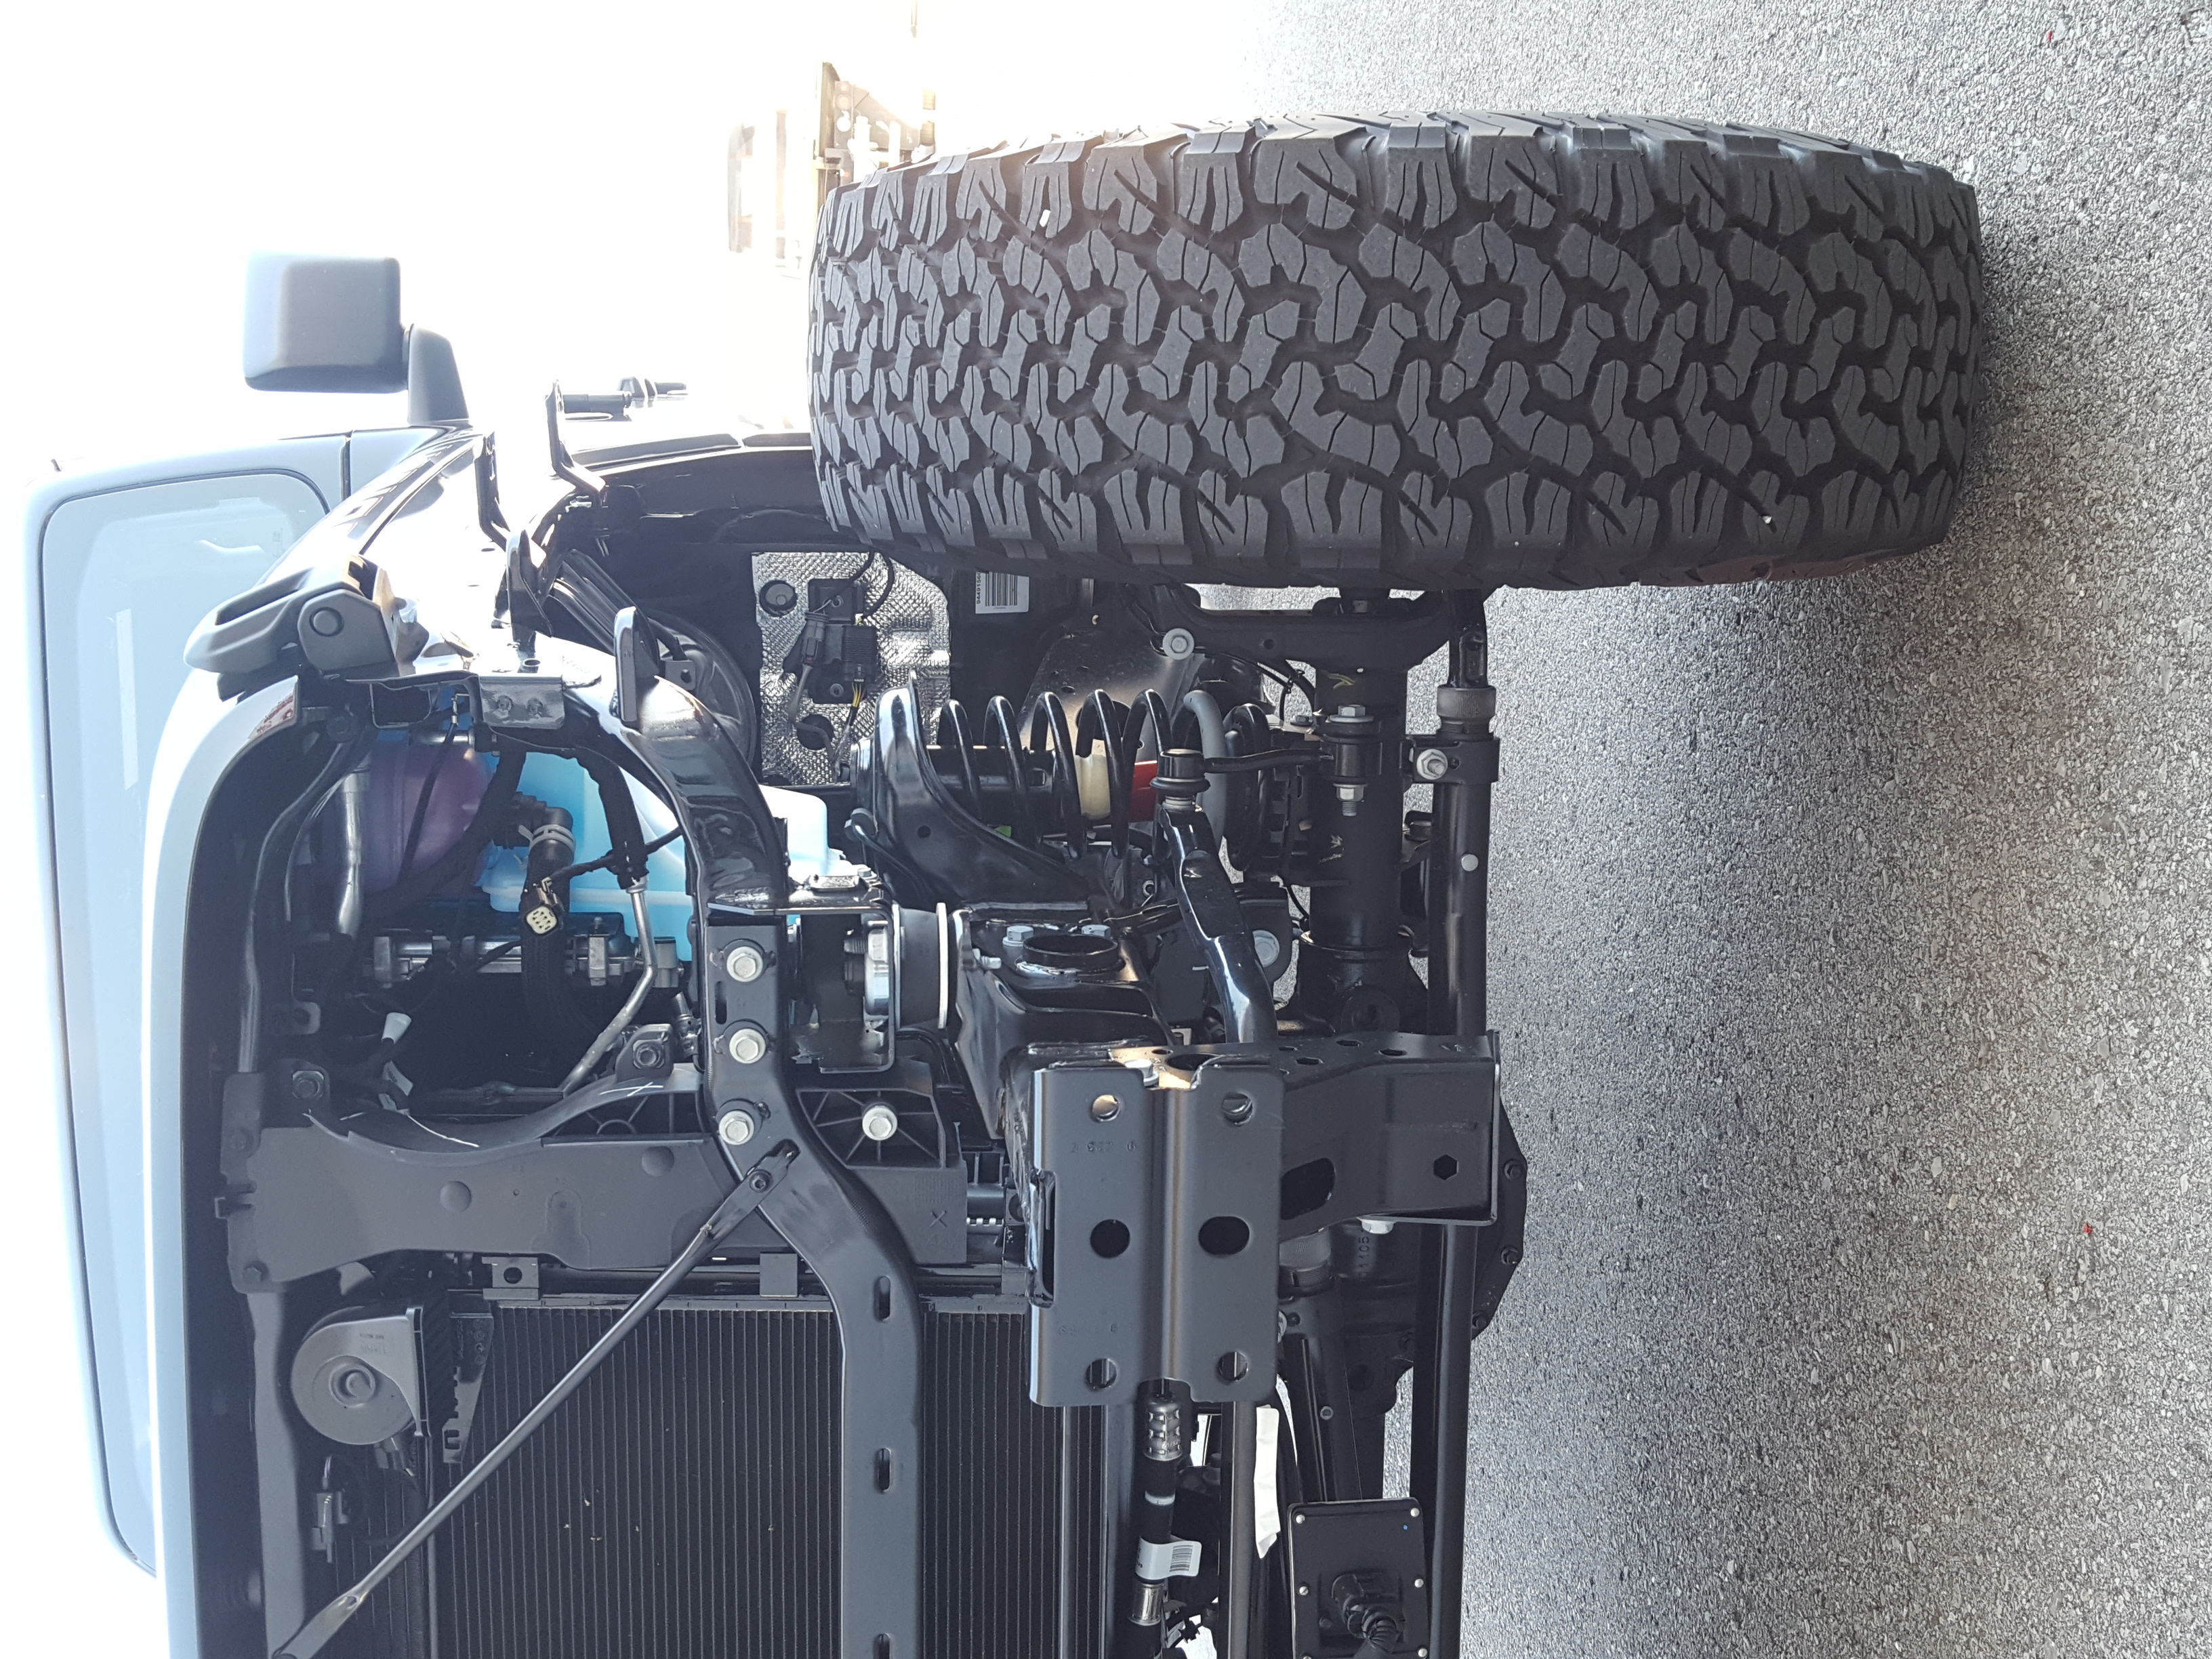
\includegraphics[scale=.05,angle=-90,origin=c]{jeep_01.jpg}	
	
	}
	
	% Section IV - Frame II	
	\frame{
		\frametitle{\sectiontitleIV \hspace{1mm} - Steps 1,2 and 3}
		
	}
	
	% Section IV - Frame III		
	\frame{
		\frametitle{\sectiontitleIV \hspace{1mm} - Steps 4,5}
		
	}	
	
\end{document}





